\section*{Oppgave 1 - Beskrivelse av produktene, markedet og kundene}
\setcounter{section}{1}
\setcounter{subsection}{0}
\addcontentsline{toc}{section}{Oppgave 1 — Markedsmiks}


\subsection{Analyse av Kviles markedssegmentering}
Kvile AS produserer robuste møbler til utendørs bruk. Høy variantbredde øker kompleksiteten i produksjon og lagerstyring, særlig når etterspørselen er sesongpreget \parencite{strandhagen2024}. Møblene produseres i Orkanger, Trøndelag, og distribueres til hele Norge. Denne seksjonen analyserer Kviles marked, kundesegmenter, produktmiks og etterspørselsmønster. Caset tar utgangspunkt i situasjonen per 1.\ november 2024.

\textbf{Kundegruppen}\\
Selskapet har tre store kunder: Statens Vegvesen, Plantasjen og Møbelringen. Vegvesenet er den største kunden målt i omsetning med 125 millioner kroner i årlig salgsvolum, mot 75 millioner til Plantasjen og Møbelringen. Vegvesenet står dermed for ca.\ 63\,\% av omsetningen, selv om antall enheter er likt (omtrent 15\,000 møbler til begge grupper). Vegvesenet betaler altså mye mer per møbel enn butikkene: 8\,333 kr (inkl.\ transport og montering på rasteplass) mot 5\,000 NOK.

\textbf{Produktmiks}\\
Kvile har fem produktserier: RAST, KVIL, KOS, KLEM og TRE. Produktvariasjonen skyldes kombinasjoner av modell, materialvalg, farge på aluminium, farge på treverk og type møbel (bord/benk). Som vist i tabell~\ref{tab:produktvarianter}, gir dette 308 SKU-er (Stock Keeping Unit) i 2024, med en økning på 96 SKU-er for hver nye aluminiumsmodell.

\begin{table}[htbp]
    \centering
    \caption[Produktvarianter per 2024]{Produktvarianter hos Kvile AS per 2024.}
    \label{tab:produktvarianter}
    \small
    \begin{tabular}{@{}lcccc@{}}
        \toprule
        \textbf{Modell} & \textbf{Alu} & \textbf{Tre} & \textbf{Typer} & \textbf{SKU-er} \\
                         & \textbf{farger} & \textbf{farger} & (bord+benk) & \\
        \midrule
        RAST (alu+tre) & 2  & 1 & 2 & 4   \\
        KVIL (alu+tre) & 6  & 8 & 2 & 96  \\
        KOS (alu+tre)  & 6  & 8 & 2 & 96  \\
        KLEM (alu+tre) & 6  & 8 & 2 & 96  \\
        TRE (kun tre)  & -- & 8 & 2 & 16  \\
        \midrule
        \multicolumn{4}{@{}l}{\textbf{Totalt 2024}} & \textbf{308} \\
        \multicolumn{4}{@{}l}{\textit{Etter ny modell 2025}} & \textit{404} \\
        \multicolumn{4}{@{}l}{\textit{Etter ny modell 2026}} & \textit{500} \\
        \bottomrule
    \end{tabular}
    
    \vspace{4pt}
    \raggedright\footnotesize
    \textit{Merk:} SKU = alu-farger $\times$ tre-farger $\times$ 2 (bord/benk). Ny aluminiummodell hvert år gir $+96$ varianter.
\end{table}

Kvile produserer rundt 30\,000 møbler i året fordelt på 308 unike produktvarianter. Volumet er for høyt til å klassifiseres som stykkproduksjon, men variasjonen gjør masseproduksjon uaktuelt. Betydelig omstillingstid på lakkanleggene gjør at Kvile må samle opp produksjon i serier av samme farge. Dette er kjennetegnet på serie-/batchproduksjon: middels volum kombinert med middels variasjon \parencite{slack2019}. Figur~\ref{fig:volum-variasjon} viser hvor Kvile plasseres i volum-variasjonsmatrisen.


% FIGUR 1: Volum vs. variasjon-matrisen

\begin{figure}[htbp]
    \centering
    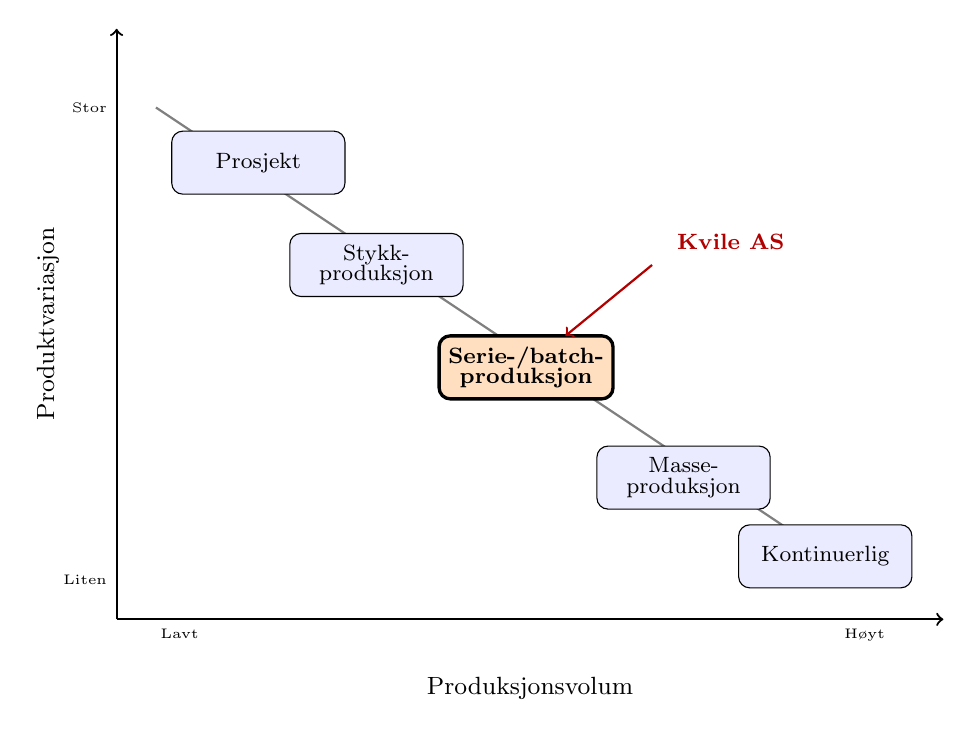
\begin{tikzpicture}[scale=1.0]
        % Akser
        \draw[->, thick] (0,0) -- (10.5,0) node[below, midway, yshift=-0.6cm, font=\small] {Produksjonsvolum};
        \draw[->, thick] (0,0) -- (0,7.5) node[above, rotate=90, midway, xshift=0cm, yshift=0.6cm, font=\small] {Produktvariasjon};
        
        % Diagonal linje
        \draw[thick, black!50] (0.5,6.5) -- (9.5,0.5);
        
        % Prosesstyper som bokser langs diagonalen
        \node[draw, rounded corners, fill=blue!8, minimum width=2.2cm, minimum height=0.8cm, font=\footnotesize] 
            at (1.8, 5.8) {Prosjekt};
        \node[draw, rounded corners, fill=blue!8, minimum width=2.2cm, minimum height=0.8cm, font=\footnotesize, align=center] 
            at (3.3, 4.5) {Stykk-\\[-2pt]produksjon};
        \node[draw, rounded corners, fill=orange!25, line width=1.2pt, minimum width=2.2cm, minimum height=0.8cm, font=\footnotesize\bfseries, align=center] 
            at (5.2, 3.2) {Serie-/batch-\\[-2pt]produksjon};
        \node[draw, rounded corners, fill=blue!8, minimum width=2.2cm, minimum height=0.8cm, font=\footnotesize, align=center] 
            at (7.2, 1.8) {Masse-\\[-2pt]produksjon};
        \node[draw, rounded corners, fill=blue!8, minimum width=2.2cm, minimum height=0.8cm, font=\footnotesize] 
            at (9.0, 0.8) {Kontinuerlig};
        
        % Kvile-markør
        \draw[->, thick, red!70!black] (6.8, 4.5) -- (5.7, 3.6);
        \node[font=\footnotesize\bfseries, red!70!black, align=center] at (7.8, 4.8) {Kvile AS};
        
        % Akselabels
        \node[font=\tiny, anchor=east] at (0, 6.5) {Stor};
        \node[font=\tiny, anchor=east] at (0, 0.5) {Liten};
        \node[font=\tiny, anchor=north] at (0.8, 0) {Lavt};
        \node[font=\tiny, anchor=north] at (9.5, 0) {Høyt};
    \end{tikzpicture}
    \caption[Volum vs.\ variasjon]{Prosesstyper: volum vs.\ variasjon. Kvile plasseres i serie-/batchproduksjon med middels volum ($\sim$30\,000 enheter/år) og middels-høy variasjon (308+ varianter). Basert på Slack \& Brandon-Jones (2019).}
    \label{fig:volum-variasjon}
\end{figure}


\textbf{Etterspørsel}\\
Etterspørselen etter Kviles produkter er preget av store sesongsvingninger, noe som er naturlig gitt at bedriften utelukkende produserer utemøbler for det norske markedet. Figur~\ref{fig:ettersporselsfordeling} illustrerer den estimerte månedlige etterspørselen fordelt på de to kundesegmentene. Vegvesenets leveranser er ordrestyrt (MTO). Bestillingene kommer minst fire måneder i forveien og gir Kvile et forutsigbart produksjonsgrunnlag, men leveransene tas kun imot i perioden mars til november. Butikkmarkedet er derimot lagerstyrt (MTS): Plantasjen og Møbelringen forventer at ferdigvarer er tilgjengelige til enhver tid, og etterspørselen fordeler seg over hele året. Likevel er det en markant sesongtopp, ettersom 50\,\% av butikksalget skjer i mai, juni og juli. Samlet gir dette en tydelig etterspørselstopp i sommermånedene, som vist i figur~\ref{fig:ettersporselsfordeling}. Det er denne sesongtoppen som gjør planleggingen vanskelig: enten må Kvile bygge opp lager gjennom lavsesongen, eller så må kapasiteten dimensjoneres for toppbelastning med mye ledig kapasitet resten av året.


% FIGUR 2: Årlig etterspørselskurve per måned (stacked)

\begin{figure}[htbp]
    \centering
    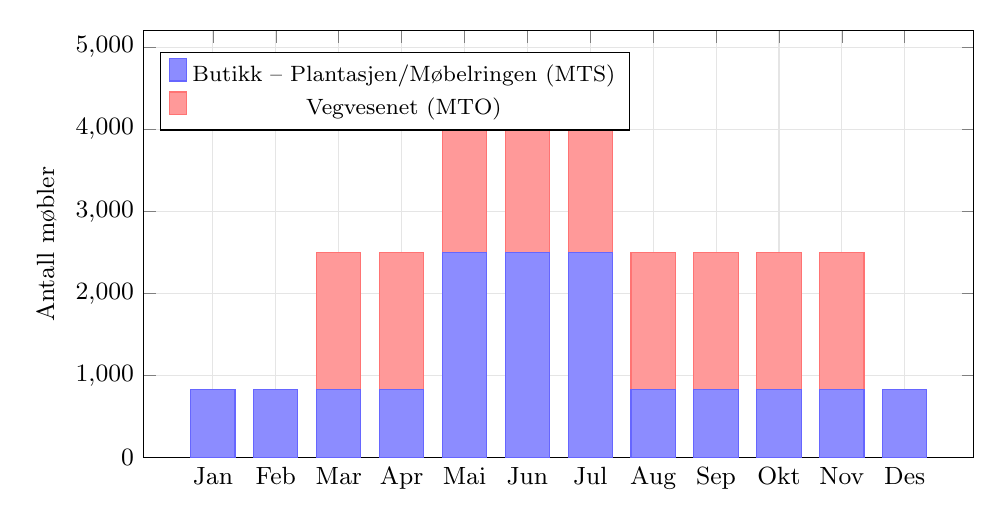
\begin{tikzpicture}
    \begin{axis}[
        width=\textwidth, height=7cm,
        ybar stacked,
        bar width=16pt,
        ymin=0, ymax=5200,
        ylabel={Antall møbler},
        symbolic x coords={Jan,Feb,Mar,Apr,Mai,Jun,Jul,Aug,Sep,Okt,Nov,Des},
        xtick=data,
        x tick label style={font=\small},
        y tick label style={font=\small},
        ylabel style={font=\small},
        legend style={at={(0.02,0.95)}, anchor=north west, font=\footnotesize},
        grid=major,
        grid style={gray!20},
    ]
    
    % Bunn: Plantasjen/Møbelringen (MTS)
    \addplot[fill=blue!45, draw=blue!60] coordinates {
        (Jan, 833)
        (Feb, 833)
        (Mar, 833)
        (Apr, 833)
        (Mai, 2500)
        (Jun, 2500)
        (Jul, 2500)
        (Aug, 833)
        (Sep, 833)
        (Okt, 833)
        (Nov, 833)
        (Des, 833)
    };
    
    % Topp: Vegvesenet (MTO)
    \addplot[fill=red!40, draw=red!55] coordinates {
        (Jan, 0)
        (Feb, 0)
        (Mar, 1667)
        (Apr, 1667)
        (Mai, 1667)
        (Jun, 1667)
        (Jul, 1667)
        (Aug, 1667)
        (Sep, 1667)
        (Okt, 1667)
        (Nov, 1667)
        (Des, 0)
    };
    
    % Usynlig serie for å plassere total-labels over søylene
    \addplot[
        draw=none, fill=none,
        nodes near coords={\pgfmathprintnumber[fixed, precision=0]{\pgfplotspointmeta}},
        nodes near coords style={font=\tiny\bfseries, anchor=south, yshift=1pt},
        point meta=explicit,
    ] coordinates {
        (Jan, 0)    [833]
        (Feb, 0)    [833]
        (Mar, 0)    [2500]
        (Apr, 0)    [2500]
        (Mai, 0)    [4167]
        (Jun, 0)    [4167]
        (Jul, 0)    [4167]
        (Aug, 0)    [2500]
        (Sep, 0)    [2500]
        (Okt, 0)    [2500]
        (Nov, 0)    [2500]
        (Des, 0)    [833]
    };
    
    \legend{Butikk -- Plantasjen/Møbelringen (MTS), Vegvesenet (MTO)}
    \end{axis}
    \end{tikzpicture}
    \caption[Månedlig etterspørsel]{Estimert total månedlig etterspørsel for Kvile AS (2023-tall). Tallene over søylene viser samlet etterspørsel fra begge segmenter. Totalvolum: $\sim$30\,000 møbler per år.}
    \label{fig:ettersporselsfordeling}
\end{figure}


